\chapter{Recursion}\index{recursion}

\section{Recursive Definitions}

\begin{defn}\index{recursive form}
  \textbf{Recursive form} defines a set, an equation, or a process by defining a starting set or a value and giving a rule for continuing to build the set, equation, or process based on previously defined terms.
\end{defn}

The key for recursion is the \emph{rule for continuing to build} the set, equation, or process. This is what allows us to do the new element, new equation, or new process based on previously defined terms.

A recursive definition has two parts.

\begin{defn}
  In the \textbf{basis step}\index{basis step}, we must define values for some finite number of
  elements. For sets, we state the \emph{basic building blocks}\index{basic
  building blocks} of the set. for functions, state the values of the function
  on the basic building blocks.
\end{defn}
\begin{defn}
  The remaining elements in the recursive definition are defined by the
  \textbf{recurrence relation}\index{recurrence relation}. For sets, we show how
  to build new things from the old with some basic construction rules. For
  functions, we show how to compute the value of a function on the new elements
  of that set.
\end{defn}

\subsection{Recursively Defined Functions}\index{functions, recursively defined}

Let us create a recursive definition of the function $F$, defined on nonnegative integers. To give a recursive definition of $F$:
\begin{enumerate}\item \emph{Basis}. Specify F(0).
    \item \emph{Recursive step}. Give a rule for defining $F(n+1)$ from $F$ evaluated at smaller values.
\end{enumerate}
\begin{ex}
  \begin{align*}
    f(0) &= 1 \\
    f(n) &= f(n-1) +2
  \end{align*}
\end{ex}
\begin{ex}
  \begin{align*}
    g(0) &= 1 \\
    g(k+1) &= g(k)+2
  \end{align*}
\end{ex}
\begin{ex}
  \begin{align*}
    a_0 &= 1 \\
    a_n &= a_{n-1}
  \end{align*}
\end{ex}
\begin{ex}
  Find the recursive form of $n!$, the function given by
  \begin{equation}\label{eq:nfact}
   n!=\prod_{k=1}^n k \
  \end{equation}
  \begin{figure}[h]
    \begin{center}
      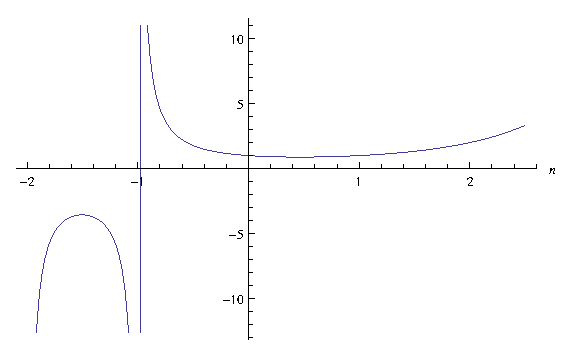
\includegraphics{discrete/recursion/nfact.eps}
    \end{center}
    \caption{A plot of $n!$. Its behavior is much harder to describe in the
    negatives, so we normally just treat it as having a domain of $n \geq 0$.}
    \label{fig:nfact}
  \end{figure}
  \begin{sol}
    The basis step in either the \emph{closed form} or \emph{recursive form}
    definition for $n!$ is that $0!=1$. In equation \eqref{eq:nfact}, it is implied
    under the convention that the product of no numbers at all is
    one\footnote{This is called the \textbf{empty product} or \textbf{nullary
    product}, and is responsible for providing the \emph{multiplicative
    identity} $1$.}

    So in order to define a recursive form for $n!$, we must start with the
    definition:
    \begin{equation}
      f(n) =
      \begin{cases}
        1 & \text{if }n=0
      \end{cases}
    \end{equation}

    Now that we have the basis step, to get the \emph{recursive step} we will
    look at a few instances of the factorial function:
    \begin{align*}
      f(0) &= 1 \\
      f(1) &= 1 \\
      f(2) &= 2 \\
      f(3) &= 6 \\
      f(4) &= 24 \\
      f(5) &= 120 \\
      & \vdots
    \end{align*}
    If we are careful, we'll notice that we can factor a $n$ from our result on
    each instance.
    \begin{align*}
      f(1) &= 1\cdot1 \\
      f(2) &= 2\cdot1 \\
      f(3) &= 3 \cdot 2 \\
      f(4) &= 4 \cdot 6 \\
      f(5) &= 5 \cdot 24 \\
      &\vdots
    \end{align*}
    We notice that $f(n)$, for any $n > 1$, is given by $n$ times the term
    before it. By writing this out, we get our \emph{recursive definition for
    factorials}.
    \begin{equation}
      f(n) =
      \begin{cases}
        1 & \text{if }n=0 \\
        n \times f(n-1) & \text{if }n > 0
      \end{cases}
    \end{equation}
    As is the case with factorials, \emph{recursive form} often offers the
    advantage that it is very intuitive for humans to understand. Its downside is
    that it is very seldom computationally faster than its \emph{closed-form}
    alternative. For this reason, we should attempt to find closed-form
    solutions to recursive definitions where possible or necessary.

    Generally speaking, given a recursive function on a test, we should be able to find a
    closed-form representation and vice-versa.
  \end{sol}
\end{ex}
\begin{ex}
  Find a recursive definition of the \textbf{Fibonacci sequence}\index{Fibonacci
  sequence}:
  \[ 1, 1, 2, 3, 5, 8 13, 21, 34, \ldots \]
  \begin{figure}[h]
    \begin{center}
      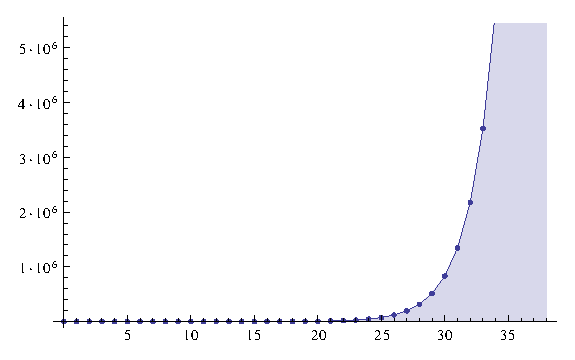
\includegraphics{discrete/recursion/fibonacci.eps}
    \end{center}
    \caption{A plot of the Fibonacci sequence.}
    \label{fig:fibonacci}
  \end{figure}

  The Fibonacci sequence is often explained using the analogy of rabbits on an
  island.
  \begin{quote}
    ``A young pair of rabbits (one for each sex) is placed on an island. After
    they are 2 months old, each pair of rabbits produces another pair each month.
    The number of pairs of rabbits after $n$ months is $f(n)$.''
  \end{quote}
  \begin{sol}
    Notice that we need \textbf{two} initial conditions to define this
    recurrence relation.
    \begin{equation}
      f(x) =
      \begin{cases}
        1 & \text{for }0 \leq x \leq 1 \\
        f(n) + f(n-1) &\text{for } x > 1
      \end{cases}
    \end{equation}
  \end{sol}
  \begin{note}
    This definition requires two initial conditions. It is very important in recursive definitions to have the right number of initial conditions.
  \end{note}
\end{ex}
%\begin{ex}
%  Give a recursive definition of
%  \[ F(n) = a^n \]
%
%  \begin{tabular}{ll}
%    $f(0)=a^0=1$ & basis \\
%    $f(n)=a\cdot f(n-1)$& recursion \\
%  \end{tabular}
%  \begin{note}
%    \[f(n)=a^n=\underbrace{a \cdot a \cdot a \cdot \dots a}_{n}\]
%
%    \[f(n-1)=a^{n-1}=\underbrace{a \cdot a \cdot a \cdot \dots a}_{n-1}\]
%  \end{note}
%\end{ex}
%\begin{ex}
%  Give a recursive definition of
%  \[ F(n) = \sum^{n}_{k=0} a_k \]
%
%  \begin{tabular}{ll}
%    $f(c)=a_0$ & basis \\
%    $f(n)=f(n-1)+a_n$ & recursion \\
%  \end{tabular}
%  \begin{note}
%    \[ F(n) = \sum^{n}_{k=0} a_k=a_0+a_1+\dots+a_{n-1}+a_n \]
%  \end{note}
%\end{ex}
%
%\begin{comment}
%\begin{ex}
%  \begin{tabular}{ll}
%    Basis. & $f(0)=100,000=A$ \\
%    Recursion. & $f(k)=f(k-1)+f(k-1)*4\%$ \\
%    & $f(k) = (1+\alpha)(f(k-1))$ \\
%  \end{tabular}
%  \begin{tabular}{ll}
%
%  \end{tabular}d
%  \end{ex}
%\end{comment}
%
%  Mathematical induction is a way to varify the correctness of a recursive definition.
%
%  \begin{ex}
%    \begin{align*}
%      a_1&=1 \\
%      a_n&=2a_{n-1}+1 \text{ for all integers n $\geq 2$}
%      \intertext{Then prove by induction:}
%      a_n&=2^n-1 \text{ for all } n \geq 1
%    \end{align*}
%    \begin{tabular}{ll}
%      & $a_1=2^1-1=1=a_1 \text{ by recursion}$\\
%      & If $a_n=2n-1$, then $a_{n+1}=2^{n+1}-1$. \\
%      & assume $a_n=2^n-1$ \\
%      & $a_{n+1}=2a_n+1=2(2^n-1)+1$ \\
%      & $= 2 \cdot 2^n -2 +1 = 2^{n+1}-1$
%    \end{tabular}
%  \end{ex}
%
%\section{Recursive Algorithms}
%
%Recursive algorithms are only used because certain algorithms are recursive in nature. Recursion does not save any computational power. For most algorithms, we can define a non-recursive version. However, sometimes it is inconvenient to find a non-recursive equivalent to a recursive algorithm.
%
%A recursive algorithm is one which calls itself to sove ``smaller'' versions of an input problem. Some algorithms are recursive in nature, like the binary search or Fibonacci sequence.
%
%The current status of the algorithm is placed on the \emph{stack}. A stack is a data structure from which entries can be added and deleted only from one end.
%
%\begin{verbatim}
%  procedure factorial(n)
%    if n < 0 return 'error'
%    if n = 0 the nreturn 1
%    else
%      return (n*factorial(n-1))
%\end{verbatim}
%
%Say we want to calculate $f(3)$.
%
%\begin{align*}
%  f(3)=3 \cdot &f(2)&&\\
%  &\to f(2) = 2 \cdot f(1)&\\
%  &&\to f(1)=1\cdot &f(0)\\
%  &&&\to f(0)=1
%\end{align*}
%
%
%
